% !TEX root = document.tex


\chapter{Editor Services}
\label{chap:editor-services}

The main subject of this thesis is what we call `Code Exploration Services'.
However, we think that we cannot discuss Code Exploration Services without first talking about the concept that forms the foundation of that idea.
That foundation is Editor Services, which is what this chapter is about.
In it we will first define what editors, and editor services are, after which we go over what it takes to implement editor services.
We finish with something called the \ac{IDE} portability problem, which is a problem central to the rest of this thesis.

\section*{}

Although programmers used to manually punch their programs into paper punchcards,
or before that, even changing the wiring of a computer just to program it, this is no longer common practice.
Instead, programmers write computer programs \emph{for} a computer, \emph{on} a computer, using a computer program commonly called an \emph{editor}.
Using editors to make new programs makes programming much faster, and vastly more accessible, essentially to everyone who has a computer.

Early on, there was \emph{ed}~\autocite{ed}, short for `editor'.
ed was one of the standard tools included on all unix operating systems, and can still be used on many modern computers.
However, ed was not very user-friendly, and is infamous for its error codes.
For all kinds of different errors, ed simply prints a \texttt{?} without any further context.

Since then, a lot has changed, and editors have become significantly more advanced.
First with editors like \emph{vi}, \emph{vim} and \emph{emacs}, which were an improvement in user experience, if only for the
fact that these allow their users to see the document while they are editing it, a feature \emph{ed} notably lacked.
Still later, \ac{GUI} editors like entered the scene.
You might know \emph{Notepad}, \emph{Notepad++} or \emph{Sublime Text}, though many more exit.
Although much more sophisticated than ed, many people would consider the examples given sofar are merely `simple text editors'.
%Many would consider these examples `simple' editors,1
%they often provide certain services to help their users,
%such as colour different parts of programs based on their syntactical meaning.

there are also more sophisticated editors, which help programmers while they write their programs, such as \emph{IntelliJ}, \emph{Eclipse} and \emph{Visual Studio Code}.
These often get called \acfp{IDE}, referring to the fact that they allow users to do much more than just edit source code
\footnote{Of course, some `simple' editors like vim and emacs can be extended near endlessly by users to feel more like an \ac{IDE}. Many people, in fact, swear by these editors, considering any added features nothing more than a distraction.}.
What makes an \ac{IDE} more sophisticated, is that an \ac{IDE} often knows much more about the language that is being edited in them and can help programmers with writing their program.
For example, an \ac{IDE} may know about the different libraries you use or might want to use, and can refer to those libraries' documentation while the programmer uses items from them in your program.

To talk about the capabilities of an \ac{IDE}, we can talk about what is called an \emph{Editor Service}, a term first used in literature by \textcite{KatsKV08}.
We can say that a `smart' editor such as an \ac{IDE}, provides many \emph{editor services} to help programmers write their programs.
However, as we will see, some things we classify as an `editor service' can also be found in many editors often considered `simple' editors, not \acp{IDE}, making the distinction between an \ac{IDE} and simpler editors a bit fuzzy\footnote{This is made worse because \ac{IDE} is sometimes used as a marketing term}.

\section{An overview of editor services}
\label{sec:an-overview-of-editor-services}

Editor services, the tools which editor provide, vary widely in kind and capability between different editors.
Nevertheless, attempts have been made to list the different kinds, based on the different kinds of services provided by many editors and \acp{IDE}.
One such list is the one by \textcite{ErdwegSV13} in \citetitle{ErdwegSV13}.
Here, a feature model for a \emph{language workbench} is given, which we will say more about in \cref{subsec:language-workbenches}.

What is important is that there is a clear relation between language workbenches and editor services.
In fact, the feature model considers it one of six main features of what a language workbench is.
Therefore, as part of defining what a language workbench is, they also list categories of editor services.

The feature model by \citeauthor{ErdwegSV13} was later adapted by \citeauthor{Pelsmaeker2018} into a list of just editor services~\autocite{Pelsmaeker2018}.
Their derived list further splits the services into larger categories, and also renames a few to sound more intuitive.
For example, syntax highlighting was renamed to syntax colouring as highlighting would imply a change in background colour.
Finally, \citeauthor{Pelsmaeker2018} also provides a useful overview of many popular editors and lists which editor services each supports.

Based on these two sources, \citeauthor{ErdwegSV13} and \citeauthor{Pelsmaeker2018}, we compiled the following list of editor services, together with a short explanation of what each means.

\paragraph{Syntax colouring}
Assigning different parts of a program different colours based on their syntactical meaning.
This depends on the language that is being written in, which can sometimes change within a document.
For example, SQL queries inside code have a different syntax from the programming language surrounding the query.
A related concept is semantic highlighting\footnote{Which should maybe be called Semantic Colouring, just like Syntax Colouring},
where colours are not assigned based on syntactical meaning, but based on semantic meaning.
For example, by giving all uses of a variable the same colour.
To provide this service for a language, an editor needs to know the syntax of that language and a colour scheme that assigns certain syntactical elements those colours.

\paragraph{Code folding}
Hiding parts of a program to reduce visual clutter.
Often this is presented to users as collapsable blocks of text, based on the syntactical meaning of that block.
For example, the body of a function or the contents of a conditional expression.
To provide this service for a language, an editor needs to know about certain points in the syntax of a language where logical blocks start.
What defines a logical block may differ per language.

\paragraph{Code completion}
Suggesting ends of words and lines as a programmer is writing.
Simple code completion can be based on occurrences of words in the same document, or project, a technique often employed by simpler editors.
This method often finds nonsensical completions.
More sophisticated code completion can involve knowledge about a languages scoping and importing rules, suggesting only completions that are valid based on context.
Recently, AI-based code completion has also established itself, with programs such as Github Copilot~\autocite{copilot} and large language models.
These tools provide completion based on a training set containing code written by others, which has sparked some debates related to whether some advanced code completion could at some point be considered plagiarism.
In fact, lawsuits~\autocite{copilot_lawsuit} have been filed over this, though no final verdict has been given at the time of writing.
To provide this service for a language, an editor needs to know about all items in scope at the location where the programmer writes, and be able to select likely candidates based on various factors.
These factors may involve the type of items around where the suggestion is made, what values are syntactically valid and what the programmer has already typed which may be a prefix of what they want the completion to be.

\paragraph{Outline}
An overview of the high-level structure of a program, like an index.
Such an overview often displays what function, class and interface names are defined in a file, and might allow quick navigation to the definition sites.
To provide this service for a language, an editor needs a simple model of the syntax of a language.
This model must have enough context to work out what items are present which are important enough to be included in the outline, and whether one such important item is nested inside another.

\paragraph{Code navigation}
Sometimes called reference resolution; resolving definition and usage sites of identifiers in programs, and providing quick navigation between these locations.
For example, finding all usages of a variable or a function.
Often, this is paired with a system to allow quick navigation between these sites, allowing quick exploration of a program.
To provide this service for a language, an editor needs, for every identifier in the program, a list of related locations in the program.
These relations between locations, in essence, form the edges in a graph where nodes are source locations.
Possibly, edges in this graph can also contain information obout what kind of relation is represented.
For example, different kinds of edges may relate a variable to other usages of that variable, or to the initial definition of a variable.

\paragraph{Documentation}
A broad range of services that attempt to match documentation with code, to make accessing documentation easier.
Examples include showing documentation of items when interacting with item names such as hovering over them,
applying markup to documentation text embedded in code and linking to online documentation.
To provide this service for a language, an editor needs the documentation for all items in a program which have documentation available.
This documentation does not necessarily need to be separately stored.
If documentation is part of source code itself, the editor could dynamically load relevant documentation by following references to definition sites which can be found through code navigation.

\paragraph{Signature help}
Especially in strongly typed languages, showing the types of an items definition while writing down a usage of that item.
For example, while writing a function call, showing the expected parameter types.
This can be related to documentation in more weakly typed languages, where types are sometimes part of comments or annotations that are essentially equivalent to comments.
Some editors might even go a step further, and will provide interactively fillable fields when items
To provide this service for a language, an editor needs to know the type signature of items in the program.

\paragraph{Automatic formatting}
Rewriting source code to match certain style guides.
Languages sometimes define standardised style guides, such as PEP8~\autocite*{pep8} and Rustfmt~\autocite{rustfmt}.
To provide this service for a language, an editor needs to know about such style guides for languages, and must then be able to apply those rules to change unformatted code into formatted code with precisely the same meaning.

\paragraph{Rename refactoring}
Automatic renaming based on context and scoping rules of language.
This is sometimes called structural search and replace~\autocite{jetbrains_ssr}.
This service is closely related to code navigation, and to provide this service for a language, an editor needs the ability to rename a single
identifier and all related identifiers from the list of related items.

\paragraph{Code actions}
A broad range of language-specific actions and transformations that can be applied to programs.
Different languages might have different code actions that make sense.
A language that has syntactical macros might allow users to expand macro usages through a code action.
As such, to provide code actions for a language, an editor needs the ability to execute language-specific actions and transformations on user-selected code.

\paragraph{Diagnostic messages}
Showing feedback, maybe from a compiler or linter, often as an overlay on source code.
To provide this service for a language, an editor needs to interpret the output of external static analysis tools (which could be a compiler).

\paragraph{Debugging}
Allowing a programmer to debug a program by showing the runtime state of that program together with the source text in the editor.
For example, displaying the location in the source code that is currently being executed and overlaying the value of variables.
To provide this service for a language, an editor needs debug symbols associated with a program that is being debugged as well as information on how to display runtime values.
However, in practice an editor might simply interface with a dedicated debugger program like \emph{gdb} and provide a graphical user interface to interact with the debugger to programmers.

\paragraph{Testing}
Showing the status of tests, and allowing users to run tests by selecting them in the editor.
To provide this service for a language, an editor needs to interpret the output of specific testing tools for that language.
Sometimes such tools are standardised like in rust, for example, which has a built-in test runner.
However, in C there is no such standard test runner, and the editor may need to support multiple different testing tools for a single language.

\section{Implementing editor services in editors}\label{sec:implementing-editor-services-in-editors}

To provide editor services, an editor needs information about the language it is providing services for.
Exactly what kind of information depends on the service.
For example, for an editor to support syntax highlighting for a language, the editor needs knowledge about the language's syntax, which might be derived from a grammar specification.

A service that only needs syntactical knowledge about a language might be considered relatively simple though.
Providing diagnostic messages, code navigation and code completion interactively might require constantly re-running analyses on source code while a user is typing, which can be enormously costly.
Although such analyses should give outputs that closely resemble that of what a compiler would show, a regular compiler is most likely not the right tool for this job\footnote{An interpreted language might not have a \emph{compiler}. However, an interpreter performs many of the steps relevant for this argument. Source code still needs to be parsed, and typechecked (even though that may happen at runtime for some languages).}.

A regular compiler, also called a \emph{batch compiler}, should be good at turning large batches of (probably mostly valid) source code into machine code quickly~\autocite{Katzan69mod, matkladlsp}.
These batches are, for example, an entire code base and its dependencies.
In contrast, the kind of program that analyses source code for an editor has different goals.
In editors, users mostly care about getting as much feedback as possible, as quickly as possible after making small changes to a program.

We will call such a compiler an `editor compiler', although that is not an established term\footnote{It is debatable if compiler is the right word for this kind of tool. An editor compiler does have to solve similar problems to batch compilers, but in the end no machine code is compiled.}.
A user expects an editor compiler to give feedback while they type, with latencies of at most a few seconds.
Often, the only way to achieve these latency goals, is by being extremely incremental, caching as much information from previous analyses to provide real-time feedback.

Furthermore, an editor compiler is often expected to be very resilient to errors.
As a user writes a program, they often leave the program in a syntactically invalid state halfway through typing a line.
Still, services such as code completion are expected to provide reasonable suggestions for these half-written programs.

And yet, an editor compiler still has much of the complexity a regular compiler has to deal with.
It still has to parse, and type check a language in a manner that is often expected to be consistent with what the regular compiler for that language would produce.
Therefore, implementing such tools can be a complex task.

\section{The \acs{IDE} Portability Problem}\label{sec:ide-portability-problem}

Because editors need knowledge about a language to provide editor services for that language, not even the most advanced editor can support all languages.
Especially lesser used languages and \acp{DSL} often have poor support from editors out of the box.
For that reason, many editors provide a way to be extended by users, often in the form of a plugin system.
That way, an author of a new language can also create a plugin providing support for that language in a specific editor,
which means the editor authors do not need to spend time supporting all languages.

However, shifting the responsibility like this creates a new problem.
Now a language author, or the community around a language, becomes responsible for providing plugins for their languages in all kinds of editors, which often work subtly different.
Again, this means that smaller languages and \acp{DSL} will be inherently less supported as they may not have the resources to implement and maintain specific tooling for multiple editors.
This problem of responsibility, where either a language has to support $n$ editors or an editor has to support $m$ languages, has been called the \ac{IDE} portability problem by \textcite{KeidelPE16}.
However, sometimes the problem is simply referred to as the \problem{\times} problem as there have to be \problem{\times} implementations providing editor services for $m$ languages and $n$ editors.

\begin{figure}
    \centering
    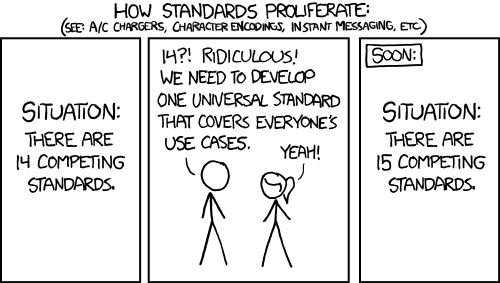
\includegraphics[width=0.65\textwidth]{../images/standards}
    \caption{XKCD `Standards', from \url{https://xkcd.com/927/}}
    \label{fig:standards}
\end{figure}

In~\citetitle{Pelsmaeker2018}, \textcite{Pelsmaeker2018} investigates this issue, and proposes a possible solution: \ac{AESI}.
\ac{AESI} is a system to create editor plugins, motivated by the desire to separate concerns between the Spoofax language workbench, and the editors supported by Spoofax.
They come up with a kind of common interface through which languages and editors can talk.
If all editors only need to support one interface to talk to all languages, and if all languages only need to support one
interface to talk to all editors, the \problem{\times} problem is essentially transformed into an \problem{+} problem.

Although the idea of a single common standard might be good in principle, it only works when all parties agree on the same standard.
The well known XKCD comic in~\cref{fig:standards} illustrates this problem.
And yet, there does seem to be one standard for editor services that is becoming reasonably universal which we will discuss in the next section.

\subsection{Language Servers}\label{subsec:language-servers}

The idea of solving the \problem{\times} problem by providing a single standardised interface through which languages and editors can talk
is also the basis for \ac{LSP}, a protocol developed by \textcite{lsp}.
Although \ac{AESI} lacked traction, \ac{LSP} is doing rather well in this regard, with support in many editors and languages~\citeyear{lsp_support}.
Importantly, Microsoft's own Visual Studio Code, one of the most popular editors, natively supports \ac{LSP} which helped the protocol gain popularity~\autocite{popularide}.

\ac{LSP} works on a client-server model.
On one side there is the \emph{language server}, which is a program that provides language-specific implementations for various kinds of editor services.
The list of supported services is almost equivalent to our list given in \cref{sec:an-overview-of-editor-services}.
A language server usually keeps running in the background for as long as the \ac{LSP} client, often an editor is open.
This allows the language server to keep state between requests.

The \ac{LSP} client and server are two different processes.
They communicate by exchanging standardised JSON messages using \acs{JSON-RPC}.
An editor that acts as an \ac{LSP} client can dynamically make requests to the server based on the user's interaction with source code in the editor.
For example, the editor might tell the server that a file has been opened, to which the server might respond that it is analysing that file now.
These requests are asynchronous, meaning that multiple requests can be in progress at the same time, and it is even possible for the language server to make a request back to the editor.
The asynchronicity also makes sure that the editor does not have to block while waiting for requests to finish.

Although \ac{LSP} defines a communication protocol, it does not define the channel over which messages are sent.
It is possible that an editor spawns a language server as a subprocess, communicating with it over \textit{stdin} and \textit{stdout}.
However, many other communication channels could be used.
For example, Eclipse Che and Theia are web editors, which make requests to a language server over the internet~\autocite{che, theia}.
This does have the disadvantage of some added latency caused by the network.

\subsection{Language Workbenches}\label{subsec:language-workbenches}

\textcite{ErdwegSVTBCGH0L15} define that ``Language workbenches are environments for simplifying the creation and use of computer languages''.
In a language workbench such as Spoofax, users can write down a description of a language in various \acp{DSL}~\autocite{Fowler2004, KallebergV07, KatsV10a}.
Such a description may consist of syntax rules of a language, a description of how the type system of the language is supposed to work, and rules on how to generate machine code.
Then, based on this description, Spoofax can derive an entire compiler and editor, complete with editor services.

With a language workbench, the workbench itself essentially functions as a common interface between editors and languages.
If a language workbench supports deriving editor service implementations for $n$ editors, then the workbench can use its
derivation rules to generate these implementations for $m$ languages specified in the language workbench, solving the \problem{\times} problem.

Of course, only languages that have a description in the language workbench can benefit from these automatically derived editor services.
This effectively excludes most big languages, which often have a custom-made compiler.
Luckily, those bigger languages likely have the resources to create a language server or implement editor services for several editors.
However, the story is different for smaller \acp{DSL}.
For those, using a language workbench could be valuable, exactly because the workbench ensures that the language immediately has editor support.

Unfortunately, the Spoofax language workbench does not support many editors to generate editor services for.
Only Eclipse is properly supported, although attempts have been made to also support \ac{LSP}-based editors and IntelliJ~\autocite{Pelsmaeker2018}.
However, Xtext, a different language workbench can generate entire Language Server implementations based on a description of a language,
which means that a \ac{DSL} made in Xtext automatically has editor support in all editors that work with \ac{LSP}.

\section{Code search}\label{sec:code-search}

Although the list of code exploration services has its roots in a list of editor services, which itself has its roots in
frequently cited theory by \textcite{ErdwegSV13}, we actually think that one feature may be missing from the original list.
That feature is search.
That search is missing is interesting, because the feature is pretty much universally supported by editors, even `dumb' ones.
Even many websites, where we showed that often relatively few services are supported, offer advanced search options.

So why is search missing?
Search doesn't create an \problem{\times} problem

